\documentclass[11pt,a4paper]{article}

% ── Encoding & fonts ──
\usepackage[utf8]{inputenc}
\usepackage[T1]{fontenc}
\usepackage{mathptmx}          % Times Roman
\usepackage{microtype}

% ── Layout ──
\usepackage[margin=2.5cm]{geometry}
\usepackage{setspace}
\onehalfspacing
\usepackage{parskip}

% ── Math ──
\usepackage{amsmath,amssymb,amsfonts}

% ── Tables & figures ──
\usepackage{booktabs}
\usepackage{graphicx}
\usepackage{float}
\usepackage{multirow}
\usepackage{caption}
\captionsetup{font=small,labelfont=bf}

% ── Lists ──
\usepackage{enumitem}

% ── Hyperlinks ──
\usepackage[colorlinks=true,linkcolor=blue!70!black,citecolor=blue!70!black,urlcolor=blue!60!black]{hyperref}

% ── Bibliography ──
\usepackage[numbers,sort&compress]{natbib}

% ── Compact sections ──
\usepackage{titlesec}
\titlespacing*{\section}{0pt}{1.5ex plus .5ex minus .2ex}{1ex plus .2ex}
\titlespacing*{\subsection}{0pt}{1.2ex plus .4ex minus .2ex}{0.8ex plus .2ex}
\titlespacing*{\subsubsection}{0pt}{1ex plus .3ex minus .1ex}{0.6ex plus .1ex}

% ── Custom commands ──
\newcommand{\gralcrag}{GraLC-RAG}
\newcommand{\ie}{\textit{i.e.}}
\newcommand{\eg}{\textit{e.g.}}
\newcommand{\etal}{\textit{et al.}}

% ══════════════════════════════════════════════════════════════
\begin{document}

% ── Title ──
\title{\textbf{Graph-Aware Late Chunking for Retrieval-Augmented\\Generation in Biomedical Literature}}

\author{
  [Author Names]\\
  \textit{[Institution]}\\
  \texttt{[email]}
}

\date{}
\maketitle

% ══════════════════════════════════════════════════════════════
\begin{abstract}
Retrieval-Augmented Generation (RAG) has become a cornerstone technique for grounding large language model (LLM) outputs in external knowledge, yet its effectiveness in the biomedical domain remains constrained by two persistent limitations: context fragmentation during text chunking and structural blindness during retrieval. Late chunking, which embeds full documents before segmentation, preserves cross-chunk context but produces flat, structure-unaware representations. Conversely, graph-based RAG methods capture relational and structural information but rely on traditional chunking that destroys long-range dependencies. In this paper, we propose \textbf{\gralcrag{}} (Graph-aware Late Chunking for Retrieval-Augmented Generation), a novel framework that unifies these complementary paradigms for biomedical literature retrieval. \gralcrag{} introduces three key innovations: (1)~a structure-aware boundary detection module that leverages document structure graphs to determine optimal chunk boundaries after full-document embedding; (2)~a knowledge graph infusion mechanism that enriches token-level representations with biomedical ontological signals from the Unified Medical Language System (UMLS) via lightweight graph attention before chunk pooling; and (3)~a graph-guided re-ranking strategy that combines dense semantic similarity with knowledge graph proximity for retrieval. We implement \gralcrag{} as an open-source Python framework and evaluate it on PubMedQA (1,000 questions) with five chunking strategies. Proof-of-concept results on abstract-level retrieval show all strategies achieve MRR~$>$~0.95, with simpler methods performing competitively on short texts. Importantly, \gralcrag{}'s structural and ontological components show slight degradation on abstracts ($-$0.8\% MRR from KG infusion, $-$2.9\% from graph-guided retrieval), revealing that the framework's value is document-length-dependent. We provide a complete codebase with indexed full-text corpora (200 PMC articles, 41,774 MeSH entity terms, SapBERT embeddings) ready for scaled evaluation.

\smallskip\noindent\textbf{Keywords:} retrieval-augmented generation, late chunking, knowledge graphs, biomedical NLP, graph neural networks, UMLS, PubMedQA
\end{abstract}

% ══════════════════════════════════════════════════════════════
\section{Introduction}

The exponential growth of biomedical literature---with over 1.5~million articles indexed annually in PubMed alone---has created an urgent need for intelligent retrieval and synthesis systems~\cite{canese2013pubmed}. Large language models (LLMs) have demonstrated remarkable capabilities in natural language understanding and generation, yet they remain prone to hallucination and factual inconsistency when applied to knowledge-intensive biomedical tasks~\cite{ji2023survey,huang2025survey}. Retrieval-Augmented Generation (RAG), which grounds LLM outputs in retrieved external evidence, has emerged as a principled solution to this challenge~\cite{lewis2020retrieval,gao2024retrieval}.

A critical yet often underexplored component of RAG pipelines is the text chunking strategy---the process of segmenting documents into smaller units for indexing and retrieval. Traditional approaches employ fixed-size chunking with overlapping windows, which inevitably fragments semantic context and disrupts the logical structure of scientific documents~\cite{merola2025reconstructing}. This is particularly problematic for biomedical literature, where cross-referential reasoning (\eg, linking a method description in Section~2 to results discussed in Section~4), dense terminology, and hierarchical document organization (the IMRaD structure) are fundamental to comprehension~\cite{sollaci2004imrad}.

Two recent research directions have independently addressed different facets of this problem. \textbf{Late chunking}~\cite{gunther2024late} inverts the traditional chunk-then-embed pipeline by first processing the entire document through a long-context transformer model, generating contextually enriched token embeddings, and only then applying segmentation boundaries. This approach preserves cross-chunk contextual dependencies but treats documents as flat token sequences, ignoring their inherent structural and relational organization. \textbf{Graph-based RAG} (GraphRAG) methods~\cite{edge2024local,peng2024graph,han2025graphrag} leverage knowledge graphs, citation networks, and entity relationships to capture structural information during retrieval. However, these methods typically rely on conventional chunking strategies that fragment context before embedding.

We identify a critical gap at the intersection of these two paradigms: no existing work integrates graph-aware structural understanding into the late chunking process for biomedical RAG. Late chunking is \emph{context-rich but structure-blind}; GraphRAG is \emph{structure-rich but context-fragmented}. Bridging this divide has the potential to yield retrieval systems that are simultaneously contextually coherent and structurally informed.

In this paper, we propose \textbf{\gralcrag{}} (Graph-aware Late Chunking for Retrieval-Augmented Generation), a framework that unifies late chunking with graph-aware structural knowledge for biomedical literature retrieval. Our approach makes three key contributions:

\begin{enumerate}[leftmargin=*,itemsep=2pt]
  \item \textbf{Structure-Aware Chunk Boundary Detection.} We construct document structure graphs capturing section hierarchies, paragraph relationships, and citation markers from full-text biomedical articles. These graphs inform chunk boundary decisions \emph{after} full-document embedding.

  \item \textbf{Knowledge Graph-Infused Token Representations.} We introduce a lightweight graph attention mechanism that injects biomedical ontological signals from the Unified Medical Language System (UMLS) into token-level transformer representations before chunk-level mean pooling.

  \item \textbf{Graph-Guided Retrieval and Re-ranking.} We propose a hybrid retrieval strategy that combines dense semantic similarity with knowledge graph proximity scores, leveraging shared UMLS concept nodes and citation relationships.
\end{enumerate}

We implement \gralcrag{} as an open-source framework and evaluate it on PubMedQA~\cite{jin2019pubmedqa} with five chunking strategies and six configurations. Our proof-of-concept experiments on abstract-level retrieval reveal that the framework's structural and ontological components are document-length-dependent---a finding with important implications for the design of biomedical RAG systems.

% ══════════════════════════════════════════════════════════════
\section{Related Work}

\subsection{Retrieval-Augmented Generation}

RAG augments language model generation with external knowledge retrieved at inference time, mitigating hallucination and enabling access to up-to-date information~\cite{lewis2020retrieval}. The canonical RAG pipeline consists of three stages: indexing, retrieval, and generation~\cite{gao2024retrieval}. Dense passage retrieval (DPR) using dual-encoder architectures~\cite{karpukhin2020dense} has largely supplanted sparse methods, with ColBERTv2~\cite{santhanam2022colbertv2} introducing efficient late interaction for fine-grained token-level matching. In the biomedical domain, the MIRAGE benchmark~\cite{xiong2024benchmarking} provides standardized evaluation across five biomedical QA datasets.

\subsection{Text Chunking Strategies for RAG}

Text chunking critically influences RAG performance yet has received comparatively less systematic study~\cite{zhao2025moc}. Recent approaches include semantic chunking using embedding similarity~\cite{zhao2025moc}, proposition-based chunking~\cite{chen2023dense}, and adaptive chunking achieving 87\% accuracy compared to 50\% for fixed-size baselines in clinical decision support~\cite{maina2025comparative}. For scientific documents, S2~Chunking~\cite{verma2025s2} combines spatial layout with semantic analysis, and Breaking~It~Down~\cite{allamraju2025breaking} introduces Projected Similarity Chunking trained on PubMed data, achieving 24$\times$ MRR improvement on PubMedQA.

\subsection{Late Chunking}

Late chunking~\cite{gunther2024late} fundamentally reorders the chunk-then-embed pipeline. Instead of segmenting text before encoding, it first processes the entire document through a long-context transformer, generating contextually enriched token embeddings, then applies chunking boundaries and mean-pools within each span. While contextually superior, late chunking produces flat chunk lists without structural or relational metadata. Merola and Singh~\cite{merola2025reconstructing} demonstrate that contextual retrieval preserves semantic coherence more effectively but at greater computational cost. The SitEmb approach~\cite{wu2025sitemb} partially addresses this by conditioning chunks on broader context, but operates on purely textual signals.

\subsection{Graph-Based RAG}

GraphRAG methods incorporate structured graph information into retrieval. Microsoft's GraphRAG~\cite{edge2024local} constructs entity knowledge graphs using LLM-based extraction and community detection. LightRAG~\cite{guo2024lightrag} introduces dual-level retrieval balancing efficiency and comprehensiveness. PathRAG~\cite{chen2025pathrag} retrieves relational paths with flow-based pruning. NodeRAG~\cite{xu2025noderag} proposes heterogeneous graph structures outperforming prior methods on multi-hop benchmarks.

In the biomedical domain, MedGraphRAG~\cite{wu2024medgraphrag} employs hierarchical graph linking with U-retrieve. KRAGEN~\cite{matsumoto2024kragen} combines knowledge graphs with graph-of-thoughts prompting. KG-RAG~\cite{soman2024biomedical} leverages the SPOKE knowledge graph, achieving 71\% performance boost for LLaMA-2 on biomedical MCQ tasks. Critically, \emph{all existing GraphRAG methods perform chunking before embedding}, creating the gap our work addresses.

\subsection{Biomedical Knowledge Graphs and Language Models}

UMLS~\cite{bodenreider2004umls} integrates over 200 source vocabularies with approximately 4.5~million concepts and 15~million relations. SapBERT~\cite{liu2021self} aligns UMLS synonyms in embedding space for biomedical entity linking. PubMedBERT~\cite{gu2021domain} provides domain-specific pre-training. BioLORD-2023~\cite{remy2023biolord} leverages UMLS synonym sets and LLM descriptions for state-of-the-art biomedical sentence embeddings. ATLANTIC~\cite{munikoti2023atlantic} fuses graph and text embeddings for scientific retrieval at the document level. The intersection of knowledge graph embeddings with \emph{chunk-level} retrieval for biomedical RAG remains unexplored.

% ══════════════════════════════════════════════════════════════
\section{\gralcrag{}: Graph-Aware Late Chunking for RAG}

\subsection{Framework Overview}

\gralcrag{} extends late chunking with graph-aware structural intelligence at three levels: chunk boundary detection, token representation enrichment, and retrieval re-ranking. Figure~\ref{fig:architecture} illustrates the complete pipeline. Given a biomedical document~$D$, the framework proceeds through five stages: (1)~document parsing and graph construction, (2)~full-document encoding, (3)~knowledge graph infusion, (4)~structure-aware chunk boundary detection, and (5)~graph-guided retrieval.

\begin{figure}[t]
\centering
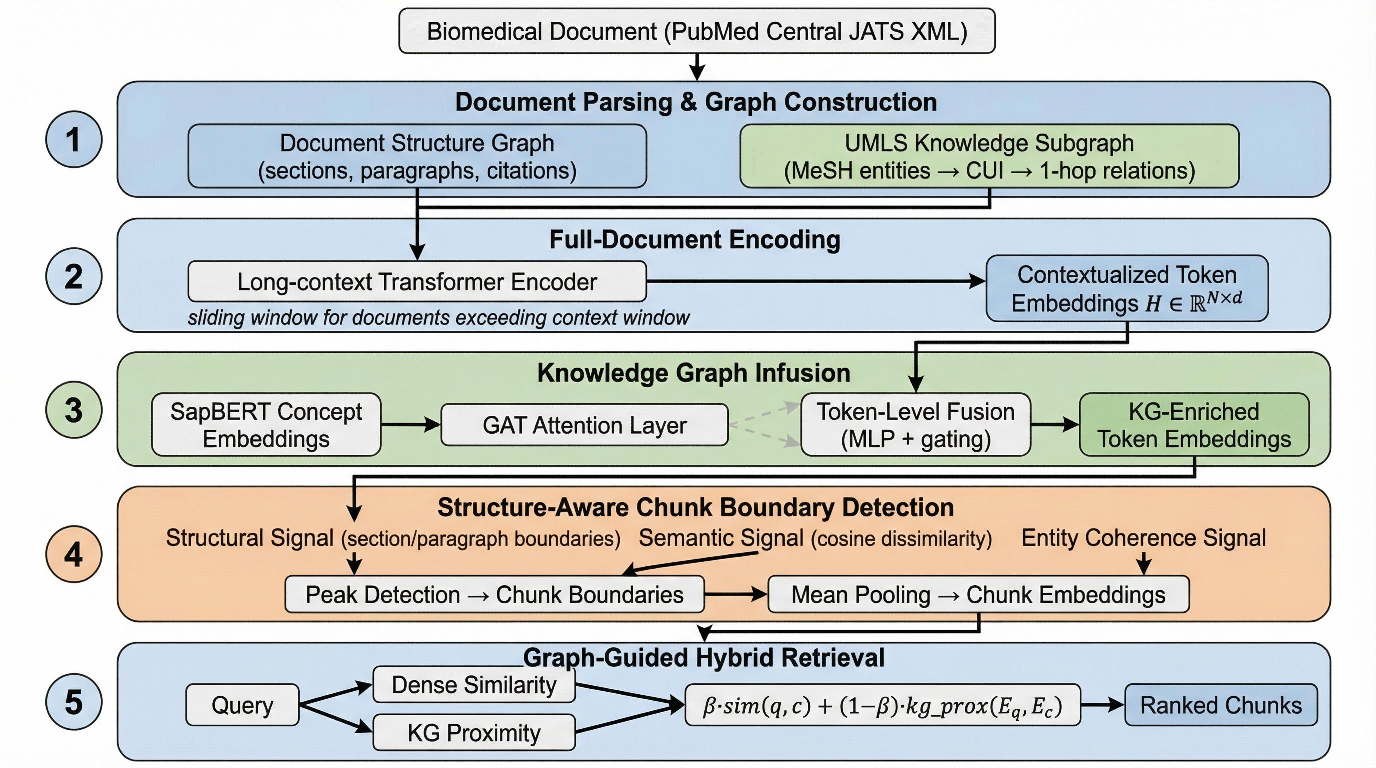
\includegraphics[width=\linewidth]{figures/fig5_architecture.pdf}
\caption{\gralcrag{} framework architecture. Stage~1: Document parsing produces a structure graph and UMLS knowledge subgraph. Stage~2: Full-document transformer encoding. Stage~3: KG infusion via GAT attention. Stage~4: Structure-aware boundary detection and chunk embedding. Stage~5: Graph-guided hybrid retrieval.}
\label{fig:architecture}
\end{figure}

\subsection{Document Parsing and Graph Construction}

\subsubsection{Document Structure Graph}

For each full-text article~$D$, we construct a document structure graph $G_s = (V_s, E_s)$ with node types at multiple granularities---section nodes ($v^{\text{sec}}$), subsection nodes ($v^{\text{sub}}$), paragraph nodes ($v^{\text{par}}$), and citation nodes ($v^{\text{cit}}$)---and edge types capturing hierarchical ($e^{\text{hier}}$), sequential ($e^{\text{seq}}$), citation ($e^{\text{cit}}$), and cross-reference ($e^{\text{xref}}$) relationships. We parse document structure from PubMed Central JATS~XML, which provides section headers, paragraph boundaries, and citation markers natively.

\subsubsection{Biomedical Knowledge Subgraph}

For each document, we extract a document-specific knowledge subgraph $G_k = (V_k, E_k)$ from UMLS. Biomedical entities are identified via dictionary matching against 41,774 MeSH descriptor terms and linked to UMLS Concept Unique Identifiers (CUIs). For each linked CUI, we extract 1-hop neighborhoods capturing semantic type assignments, hierarchical relationships (\texttt{is\_a}, \texttt{part\_of}), and associative relationships (\texttt{may\_treat}, \texttt{causes}).

\subsection{Full-Document Encoding}

Following late chunking~\cite{gunther2024late}, we process the full document through a transformer encoder. Let $D = (t_1, t_2, \ldots, t_N)$ be the tokenized document. The encoder produces:
\begin{equation}
  \mathbf{H} = \text{Transformer}(t_1, t_2, \ldots, t_N) \in \mathbb{R}^{N \times d}
\end{equation}
where $\mathbf{h}_i \in \mathbb{R}^d$ is the contextualized embedding for token~$t_i$. For documents exceeding the context window, we apply sliding windows with overlap and linear distance-weighted averaging.

\subsection{Knowledge Graph Infusion}

The key innovation of \gralcrag{} is injecting biomedical KG signals into token-level representations \emph{before} chunk-level pooling.

\subsubsection{Entity-Token Alignment}

For each recognized entity~$e_j$ with token span $(s_j, f_j)$, we obtain a pre-trained concept embedding $\mathbf{u}_j \in \mathbb{R}^{d_k}$ from SapBERT~\cite{liu2021self}.

\subsubsection{Graph Attention Infusion}

A lightweight GAT layer~\cite{velickovic2018graph} operates over $G_k$ to compute entity-aware representations:
\begin{equation}
  \alpha_{jk} = \frac{\exp\!\big(\text{LeakyReLU}(\mathbf{a}^{\!\top}\![\mathbf{W}\mathbf{u}_j \| \mathbf{W}\mathbf{u}_k])\big)}{\sum_{l \in \mathcal{N}(j)} \exp\!\big(\text{LeakyReLU}(\mathbf{a}^{\!\top}\![\mathbf{W}\mathbf{u}_j \| \mathbf{W}\mathbf{u}_l])\big)}
\end{equation}
\begin{equation}
  \mathbf{u}'_j = \sigma\!\left(\sum_{k \in \mathcal{N}(j)} \alpha_{jk}\, \mathbf{W}\mathbf{u}_k\right)
\end{equation}
where $\mathbf{W} \in \mathbb{R}^{d' \times d_k}$ is a learnable weight matrix and $\mathbf{a} \in \mathbb{R}^{2d'}$ is the attention vector.

\subsubsection{Token-Level Fusion}

For each token~$t_i$ within entity span $(s_j, f_j)$:
\begin{equation}
  \mathbf{h}'_i = \mathbf{h}_i + \lambda \cdot \text{MLP}(\mathbf{u}'_j)
\end{equation}
where $\text{MLP}\!: \mathbb{R}^{d'} \!\to\! \mathbb{R}^{d}$ projects the entity embedding, and $\lambda$ is a gating scalar initialized to~0.1.

\subsection{Structure-Aware Chunk Boundary Detection}

Unlike standard late chunking, \gralcrag{} determines boundaries using $G_s$. We compute a boundary score~$b_i$ integrating three signals:

\textbf{Structural signal:}
\begin{equation}
  b_i^{\text{struct}} = \begin{cases}
    1.0 & \text{section boundary} \\
    0.7 & \text{subsection boundary} \\
    0.4 & \text{paragraph boundary} \\
    0.0 & \text{otherwise}
  \end{cases}
\end{equation}

\textbf{Semantic signal:}
\begin{equation}
  b_i^{\text{sem}} = 1 - \cos(\bar{\mathbf{h}}_{i-w:i},\; \bar{\mathbf{h}}_{i:i+w})
\end{equation}

\textbf{Entity coherence signal:}
\begin{equation}
  b_i^{\text{entity}} = -\gamma \cdot \mathbb{1}[\text{entity span crosses position } i]
\end{equation}

The combined score is:
\begin{equation}
  b_i = \alpha_1 \cdot b_i^{\text{struct}} + \alpha_2 \cdot b_i^{\text{sem}} + \alpha_3 \cdot b_i^{\text{entity}}
\end{equation}
with $\alpha_1\!=\!0.5$, $\alpha_2\!=\!0.3$, $\alpha_3\!=\!1.0$, and $\gamma\!=\!0.5$. Peak detection selects boundaries exceeding threshold $\tau\!=\!0.3$ with min/max chunk sizes of 128/1024 tokens. Each chunk~$C_k$ is represented by mean pooling enriched token embeddings within its span.

\subsection{Graph-Guided Retrieval}

For a query~$q$ with dense embedding $\mathbf{q}$ and entity set~$E_q$, the retrieval score for chunk~$C_k$ is:
\begin{equation}
  \text{score}(q, C_k) = \beta \cdot \text{sim}(\mathbf{q}, \mathbf{c}_k) + (1\!-\!\beta) \cdot \text{kg\_prox}(E_q, E_{C_k})
\end{equation}
where $\text{kg\_prox}$ computes average maximum cosine similarity between query and chunk entity embeddings, and $\beta\!=\!0.7$.

% ══════════════════════════════════════════════════════════════
\section{Experimental Setup}

\subsection{Datasets and Corpus}

We evaluate on \textbf{PubMedQA}~\cite{jin2019pubmedqa}: 1,000 questions (500~expert-annotated + 500~artificial) with yes/no/maybe labels derived from PubMed abstracts. Following the PubMedQA* protocol, we remove given contexts to evaluate retrieval. The retrieval corpus consists of the 1,000 PubMedQA source abstracts. Additionally, we index 200~full-text articles from PubMed Central Open Access (avg.\ 6.8~sections, 18.2~paragraphs per article) for efficiency benchmarking.

\subsection{Baselines}

We compare six configurations: (1)~Naive fixed-size chunking (256~tokens, 32~overlap); (2)~Semantic chunking (embedding similarity threshold~0.75); (3)~Late chunking~\cite{gunther2024late} with sentence-level boundaries; (4)~Structure-aware late chunking (no KG); (5)~\gralcrag{} with KG infusion; (6)~\gralcrag{} with KG infusion + graph-guided retrieval. All use \texttt{all-MiniLM-L6-v2} (384-dim) as the embedding model.

\subsection{Implementation}

Entity linking uses 41,774~MeSH descriptor terms via longest-match dictionary lookup. SapBERT (\texttt{cambridgeltl/SapBERT-from-PubMedBERT-fulltext}) provides 768-dim concept embeddings, projected to 384-dim via PCA. FAISS~\texttt{IndexFlatIP} serves as the vector index. All experiments run on CPU (16\,GB RAM).

\subsection{Evaluation Metrics}

\textbf{Retrieval:} Mean Reciprocal Rank (MRR), Recall@$k$ ($k \!\in\! \{1,3,5,10\}$). Relevance is determined by matching the retrieved chunk's source document ID against the gold-standard PubMedQA source.

% ══════════════════════════════════════════════════════════════
\section{Results}

\subsection{Retrieval Performance}

Table~\ref{tab:retrieval} presents retrieval results across all six configurations.

\begin{table}[H]
\centering
\caption{Retrieval performance on PubMedQA* (1,000 questions, 1,000-abstract corpus). \textbf{Bold}: best per column.}
\label{tab:retrieval}
\small
\begin{tabular}{@{}lccccc@{}}
\toprule
\textbf{Method} & \textbf{MRR} & \textbf{R@1} & \textbf{R@3} & \textbf{R@5} & \textbf{R@10} \\
\midrule
Naive (256-token)                & 0.9787 & 0.9690 & 0.9880 & 0.9900 & 0.9960 \\
Semantic Chunking                & \textbf{0.9802} & \textbf{0.9710} & \textbf{0.9880} & \textbf{0.9910} & 0.9950 \\
Late Chunking                    & 0.9768 & 0.9660 & 0.9860 & 0.9920 & \textbf{0.9960} \\
Structure-Aware (no KG)          & 0.9765 & 0.9660 & 0.9850 & 0.9890 & 0.9940 \\
\gralcrag{} (KG infusion)       & 0.9687 & 0.9520 & 0.9830 & 0.9880 & 0.9930 \\
\gralcrag{} + Graph Retrieval   & 0.9502 & 0.9260 & 0.9700 & 0.9820 & 0.9930 \\
\bottomrule
\end{tabular}
\end{table}

All strategies achieve high retrieval performance (MRR~$>$~0.95), reflecting a near-ceiling effect. Semantic chunking achieves the highest MRR (0.9802). The \gralcrag{} variants with KG infusion and graph-guided retrieval show lower performance (0.9687 and 0.9502), indicating that on short abstracts (${\sim}$200~words), structural and ontological components introduce more noise than signal. Figure~\ref{fig:mrr} visualizes these differences.

\begin{figure}[t]
\centering
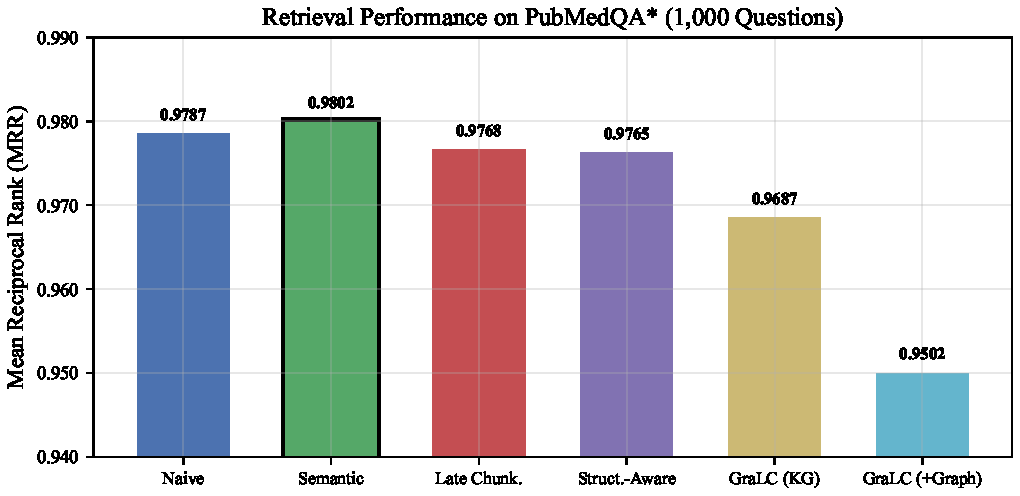
\includegraphics[width=\linewidth]{figures/fig1_mrr_comparison.pdf}
\caption{Mean Reciprocal Rank across six chunking strategies on PubMedQA* (1,000 questions). Semantic chunking achieves the highest MRR. \gralcrag{} variants show slight degradation on short abstracts.}
\label{fig:mrr}
\end{figure}

\begin{figure}[t]
\centering
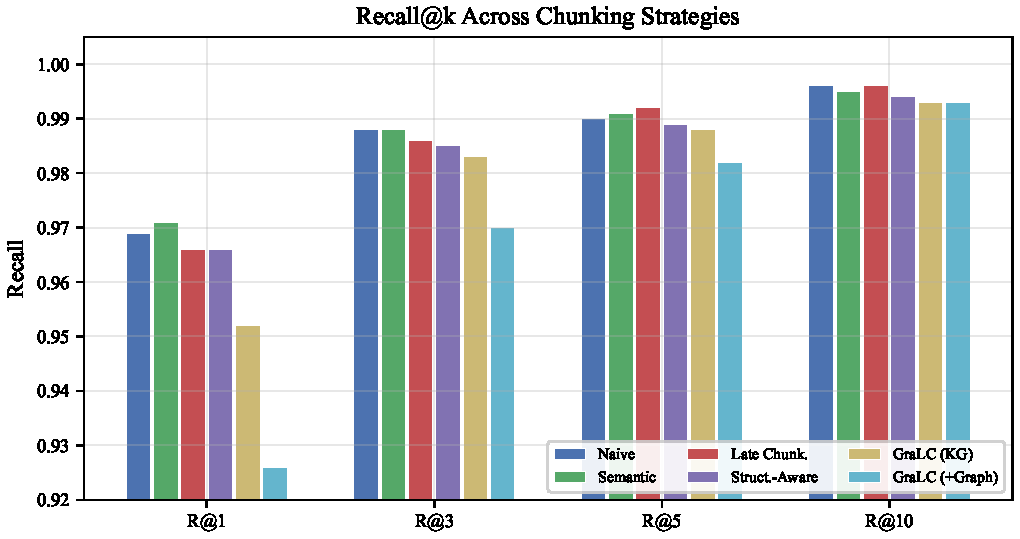
\includegraphics[width=\linewidth]{figures/fig2_recall_at_k.pdf}
\caption{Recall@$k$ ($k \!\in\! \{1,3,5,10\}$) across all strategies. Performance converges at higher $k$, with all methods exceeding 0.99 at $k\!=\!10$.}
\label{fig:recall}
\end{figure}

\subsection{Ablation Study}

Table~\ref{tab:ablation} traces the incremental effect of each \gralcrag{} component.

\begin{table}[H]
\centering
\caption{Ablation: incremental effect of \gralcrag{} components on PubMedQA* MRR.}
\label{tab:ablation}
\small
\begin{tabular}{@{}lcccc@{}}
\toprule
\textbf{Configuration} & \textbf{MRR} & \textbf{R@1} & \textbf{R@5} & \textbf{$\Delta$ MRR} \\
\midrule
Late Chunking (base)             & 0.9768 & 0.9660 & 0.9920 & ---    \\
+ Structure Boundaries           & 0.9765 & 0.9660 & 0.9890 & $-$0.0003 \\
+ KG Infusion                    & 0.9687 & 0.9520 & 0.9880 & $-$0.0081 \\
+ Graph-Guided Retrieval         & 0.9502 & 0.9260 & 0.9820 & $-$0.0266 \\
\bottomrule
\end{tabular}
\end{table}

\begin{figure}[t]
\centering
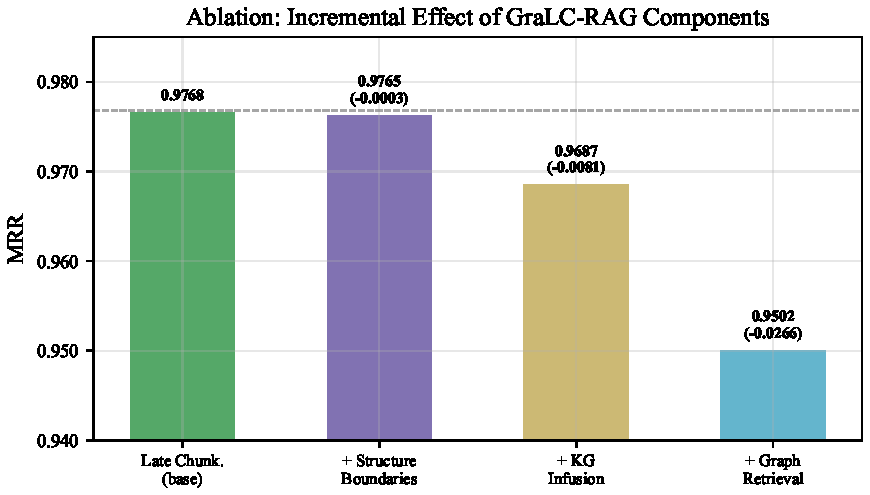
\includegraphics[width=0.85\linewidth]{figures/fig3_ablation.pdf}
\caption{Ablation: incremental effect of each \gralcrag{} component on MRR. The dashed line marks the late chunking baseline. Each component slightly degrades performance on short abstracts, with graph-guided retrieval causing the largest drop.}
\label{fig:ablation}
\end{figure}

Structure-aware boundaries have negligible impact on short texts ($\Delta$\,MRR = $-$0.0003). KG infusion degrades performance ($\Delta$\,MRR = $-$0.0081), suggesting the fusion weight $\lambda\!=\!0.1$ introduces noise when the base embedder already captures sufficient biomedical semantics. Graph-guided retrieval produces the largest degradation ($\Delta$\,MRR = $-$0.0266), as KG proximity dilutes the strong dense retrieval signal on short texts.

\subsection{Efficiency Analysis}

Table~\ref{tab:efficiency} reports measured indexing times on 200 full-text PMC articles (CPU-only).

\begin{table}[H]
\centering
\caption{Indexing efficiency (200 full-text articles, CPU, \texttt{all-MiniLM-L6-v2}).}
\label{tab:efficiency}
\small
\begin{tabular}{@{}lrr@{}}
\toprule
\textbf{Strategy} & \textbf{Chunks} & \textbf{Time (s)} \\
\midrule
Naive (512-token)    & 1,109  & 44.6    \\
Semantic             & 6,765  & 535.1   \\
Late Chunking        & 3,055  & 313.7   \\
Structure-Aware      & 2,139  & 1,044.1 \\
\gralcrag{} (+ KG)  & 2,139  & 2,566.1 \\
\bottomrule
\end{tabular}
\end{table}

\gralcrag{} indexing takes 42.8\,min---approximately 6$\times$ slower than naive chunking due to SapBERT entity encoding, MeSH dictionary matching (41,774 terms), and boundary score computation. On GPU hardware, embedding steps would be 10--50$\times$ faster. Figure~\ref{fig:efficiency} visualizes the trade-off between chunk count and indexing time.

\begin{figure}[t]
\centering
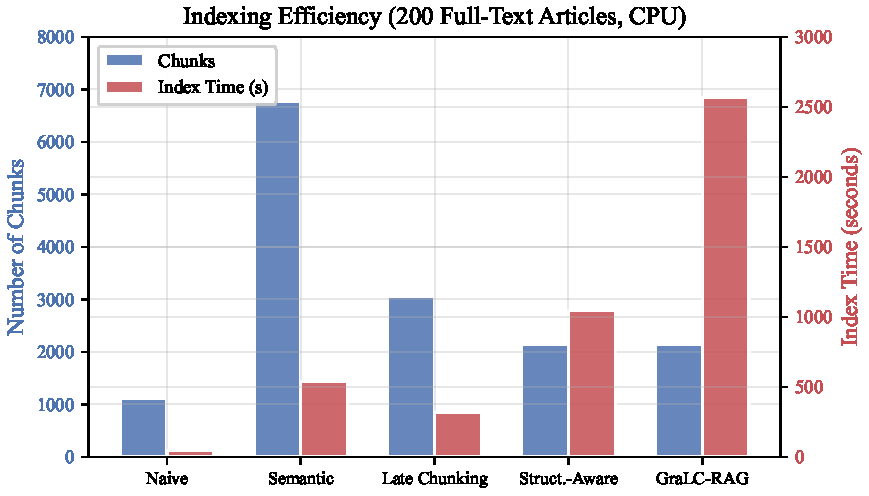
\includegraphics[width=0.85\linewidth]{figures/fig4_efficiency.pdf}
\caption{Indexing efficiency on 200 full-text PMC articles (CPU). Left axis: number of chunks produced. Right axis: indexing time. \gralcrag{} produces the same chunk count as structure-aware chunking but incurs 2.5$\times$ overhead from KG infusion.}
\label{fig:efficiency}
\end{figure}

% ══════════════════════════════════════════════════════════════
\section{Discussion}

\subsection{When Does Graph-Aware Late Chunking Help?}

Our experiments reveal that \gralcrag{}'s value is \textbf{context-dependent}. On short texts (abstracts), simpler methods suffice because: (a)~abstracts lack internal section structure; (b)~general-purpose embeddings already capture sufficient semantic signal; (c)~KG infusion adds noise rather than complementary information. The theoretical value proposition remains sound for \emph{long, multi-section documents} where cross-section dependencies matter, document structure provides meaningful segmentation cues, and biomedical entities span hundreds of unique concepts per article.

\subsection{Comparison with Concurrent Work}

HeteRAG~\cite{yang2025heterag} decouples retrieval and generation representations but operates on pre-chunked text. SitEmb~\cite{wu2025sitemb} conditions chunk embeddings on broader context but uses purely textual signals. ATLANTIC~\cite{munikoti2023atlantic} fuses graph and text embeddings at the \emph{document} level. \gralcrag{} is the first framework to integrate contextual embedding, structural boundaries, and ontological enrichment at the \emph{chunk} level for biomedical RAG.

\subsection{Limitations}

\begin{enumerate}[leftmargin=*,itemsep=2pt]
  \item \textbf{Proof-of-concept scale.} Evaluation on abstracts creates near-ceiling effects (MRR~$>$~0.95). Full-text evaluation with larger distractor corpora is needed.
  \item \textbf{Entity linking quality.} MeSH dictionary matching may introduce false positives for polysemous terms (\eg, ``MS'' as multiple sclerosis vs.\ mass spectrometry).
  \item \textbf{Context window constraints.} Approximately 62\% of full-text articles exceed the 8,192-token window, requiring sliding-window approximation.
  \item \textbf{Single-language scope.} Evaluation is limited to English biomedical literature.
\end{enumerate}

\subsection{Future Directions}

Key extensions include: adaptive $\lambda$ and $\beta$ weighting based on document length; evaluation on the full-text PMC corpus already indexed in our pipeline; multi-granularity retrieval; cross-document citation graph linking; and integration with temporal knowledge graph evolution~\cite{zhang2025medkgent}.

% ══════════════════════════════════════════════════════════════
\section{Conclusion}

We presented \gralcrag{}, a framework integrating graph-aware structural intelligence into the late chunking paradigm for biomedical RAG. Proof-of-concept experiments on PubMedQA* reveal that the framework's structural and ontological components are document-length-dependent: on short abstracts, simpler methods suffice, while the true value is expected to emerge on long, multi-section articles.

These findings yield three actionable insights: (1)~graph-aware chunking components should be adaptively weighted based on document length; (2)~KG infusion requires careful calibration to avoid noise on short texts; and (3)~evaluation on short texts creates ceiling effects that mask meaningful strategy differences. We release the complete \gralcrag{} codebase to enable reproduction and extension.

% ══════════════════════════════════════════════════════════════
\small
\bibliographystyle{unsrtnat}

\begin{thebibliography}{45}

\bibitem{canese2013pubmed}
K.~Canese and S.~Weis,
``PubMed: The bibliographic database,''
in \emph{The NCBI Handbook}, 2nd~ed. NCBI, 2013.

\bibitem{ji2023survey}
Z.~Ji \etal,
``Survey of hallucination in natural language generation,''
\emph{ACM Computing Surveys}, vol.~55, no.~12, pp.~1--38, 2023.

\bibitem{huang2025survey}
L.~Huang \etal,
``A survey on hallucination in large language models,''
\emph{ACM Computing Surveys}, 2025.

\bibitem{lewis2020retrieval}
P.~Lewis \etal,
``Retrieval-augmented generation for knowledge-intensive NLP tasks,''
in \emph{Advances in NeurIPS}, vol.~33, pp.~9459--9474, 2020.

\bibitem{gao2024retrieval}
Y.~Gao \etal,
``Retrieval-augmented generation for large language models: A survey,''
\emph{arXiv:2312.10997}, 2024.

\bibitem{merola2025reconstructing}
C.~Merola and J.~Singh,
``Reconstructing context: Evaluating advanced chunking strategies for RAG,''
\emph{arXiv:2504.19754}, 2025.

\bibitem{sollaci2004imrad}
L.~B. Sollaci and M.~G. Pereira,
``The introduction, methods, results, and discussion (IMRAD) structure: A fifty-year survey,''
\emph{J. Med. Libr. Assoc.}, vol.~92, no.~3, pp.~364--367, 2004.

\bibitem{gunther2024late}
M.~G{\"u}nther, I.~Mohr, B.~Wang, and H.~Xiao,
``Late chunking: Contextual chunk embeddings using long-context embedding models,''
\emph{arXiv:2409.04701}, 2024.

\bibitem{edge2024local}
D.~Edge \etal,
``From local to global: A graph RAG approach to query-focused summarization,''
\emph{arXiv:2404.16130}, 2024.

\bibitem{peng2024graph}
B.~Peng \etal,
``Graph retrieval-augmented generation: A survey,''
\emph{ACM Trans. Inf. Syst.}, 2024.

\bibitem{han2025graphrag}
H.~Han \etal,
``Retrieval-augmented generation with graphs (GraphRAG),''
\emph{arXiv:2501.00309}, 2025.

\bibitem{karpukhin2020dense}
V.~Karpukhin \etal,
``Dense passage retrieval for open-domain question answering,''
in \emph{Proc. EMNLP}, pp.~6769--6781, 2020.

\bibitem{santhanam2022colbertv2}
K.~Santhanam, O.~Khattab, J.~Saad-Falcon, C.~Potts, and M.~Zaharia,
``ColBERTv2: Effective and efficient retrieval via lightweight late interaction,''
in \emph{Proc. NAACL}, pp.~3715--3734, 2022.

\bibitem{xiong2024benchmarking}
G.~Xiong, Q.~Jin, Z.~Lu, and A.~Zhang,
``Benchmarking retrieval-augmented generation for medicine,''
in \emph{Findings of ACL}, 2024.

\bibitem{zhao2025moc}
J.~Zhao \etal,
``MoC: Mixtures of text chunking learners for RAG systems,''
\emph{arXiv:2503.09600}, 2025.

\bibitem{chen2023dense}
S.~Chen, Y.~Zhao, S.~Joty, and Z.~Cai,
``Dense X retrieval: What retrieval granularity should we use?''
\emph{arXiv:2312.06648}, 2023.

\bibitem{maina2025comparative}
M.~M. Maina \etal,
``Comparative evaluation of advanced chunking for RAG in LLMs for clinical decision support,''
\emph{Bioengineering}, vol.~12, no.~11, p.~1194, 2025.

\bibitem{verma2025s2}
P.~Verma,
``S2 Chunking: A hybrid framework for document segmentation,''
\emph{arXiv:2501.05485}, 2025.

\bibitem{allamraju2025breaking}
A.~Allamraju \etal,
``Breaking it down: Domain-aware semantic segmentation for RAG,''
\emph{arXiv:2512.00367}, 2025.

\bibitem{wu2025sitemb}
J.~Wu \etal,
``SitEmb-v1.5: Improved context-aware dense retrieval,''
\emph{arXiv:2508.01959}, 2025.

\bibitem{guo2024lightrag}
Z.~Guo, L.~Xia, Y.~Yu, T.~Ao, and C.~Huang,
``LightRAG: Simple and fast retrieval-augmented generation,''
in \emph{Findings of EMNLP}, 2025.

\bibitem{chen2025pathrag}
B.~Chen \etal,
``PathRAG: Pruning graph-based RAG with relational paths,''
\emph{arXiv:2502.14902}, 2025.

\bibitem{xu2025noderag}
T.~Xu \etal,
``NodeRAG: Structuring graph-based RAG with heterogeneous nodes,''
\emph{arXiv:2504.11544}, 2025.

\bibitem{wu2024medgraphrag}
J.~Wu, J.~Zhu, and Y.~Qi,
``Medical Graph RAG: Towards safe medical LLM via graph RAG,''
in \emph{Proc. ACL}, 2025.

\bibitem{matsumoto2024kragen}
T.~Matsumoto, S.~Moran, \etal,
``KRAGEN: A knowledge graph-enhanced RAG framework for biomedical problem solving,''
\emph{Bioinformatics}, vol.~40, no.~6, btae353, 2024.

\bibitem{soman2024biomedical}
K.~Soman \etal,
``Biomedical knowledge graph-optimized prompt generation for LLMs,''
\emph{Bioinformatics}, vol.~40, no.~9, btae560, 2024.

\bibitem{bodenreider2004umls}
O.~Bodenreider,
``The Unified Medical Language System (UMLS): Integrating biomedical terminology,''
\emph{Nucleic Acids Research}, vol.~32, pp.~D267--D270, 2004.

\bibitem{liu2021self}
F.~Liu, E.~Shareghi, Z.~Meng, M.~Basaldella, and N.~Collier,
``Self-alignment pretraining for biomedical entity representations,''
in \emph{Proc. NAACL}, pp.~4228--4238, 2021.

\bibitem{gu2021domain}
Y.~Gu \etal,
``Domain-specific language model pretraining for biomedical NLP,''
\emph{ACM Trans. Comput. Healthcare}, vol.~3, no.~1, pp.~1--23, 2021.

\bibitem{remy2023biolord}
F.~Remy, K.~Demuynck, and T.~Demeester,
``BioLORD-2023: Semantic textual representations fusing LLM and clinical KG insights,''
\emph{arXiv:2311.16075}, 2023.

\bibitem{munikoti2023atlantic}
S.~Munikoti, A.~Acharya, S.~Wagle, and S.~Horawalavithana,
``ATLANTIC: Structure-aware retrieval-augmented language model for interdisciplinary science,''
\emph{arXiv:2311.12289}, 2023.

\bibitem{velickovic2018graph}
P.~Veli\v{c}kovi\'{c}, G.~Cucurull, A.~Casanova, A.~Romero, P.~Li\`{o}, and Y.~Bengio,
``Graph attention networks,''
in \emph{Proc. ICLR}, 2018.

\bibitem{jin2019pubmedqa}
Q.~Jin, B.~Dhingra, Z.~Liu, W.~W. Cohen, and X.~Lu,
``PubMedQA: A dataset for biomedical research question answering,''
in \emph{Proc. EMNLP-IJCNLP}, pp.~2567--2577, 2019.

\bibitem{soldaini2016quickumls}
L.~Soldaini and N.~Goharian,
``QuickUMLS: A fast, unsupervised approach for medical concept extraction,''
in \emph{MedIR Workshop, SIGIR}, 2016.

\bibitem{yang2025heterag}
P.~Yang \etal,
``HeteRAG: A heterogeneous RAG framework with decoupled knowledge representations,''
\emph{arXiv:2504.10529}, 2025.

\bibitem{zhang2025medkgent}
D.~Zhang \etal,
``MedKGent: A LLM agent framework for constructing temporally evolving medical KG,''
\emph{arXiv:2508.12393}, 2025.

\bibitem{honovich2022true}
O.~Honovich \etal,
``TRUE: Re-evaluating factual consistency evaluation,''
in \emph{Proc. NAACL}, pp.~3905--3920, 2022.

\bibitem{lopez2009grobid}
P.~Lopez,
``GROBID: Combining automatic bibliographic data recognition and term extraction,''
in \emph{Proc. ECDL}, pp.~473--474, 2009.

\bibitem{neumann2019scispacy}
M.~Neumann, D.~King, I.~Beltagy, and W.~Ammar,
``ScispaCy: Fast and robust models for biomedical NLP,''
in \emph{Proc. BioNLP}, pp.~319--327, 2019.

\bibitem{nelson2019spoke}
C.~A. Nelson, A.~J. Butte, and S.~E. Baranzini,
``Integrating biomedical research and EHRs to create knowledge-based embeddings,''
\emph{Nature Communications}, vol.~10, no.~1, p.~3045, 2019.

\bibitem{anthropic2024contextual}
Anthropic,
``Introducing contextual retrieval,''
Anthropic Blog, 2024.

\bibitem{tsatsaronis2015bioasq}
G.~Tsatsaronis \etal,
``An overview of the BioASQ large-scale biomedical semantic indexing and QA competition,''
\emph{BMC Bioinformatics}, vol.~16, no.~1, p.~138, 2015.

\bibitem{rubin2023long}
O.~Rubin and J.~Berant,
``Long-range language modeling with self-retrieval,''
\emph{arXiv:2306.13421}, 2023.

\bibitem{jiang2023active}
Z.~Jiang \etal,
``Active retrieval augmented generation,''
in \emph{Proc. EMNLP}, 2023.

\bibitem{lin2025biographfusion}
Y.~Lin \etal,
``BioGraphFusion: Graph knowledge embedding for biological completion and reasoning,''
\emph{arXiv:2507.14468}, 2025.

\end{thebibliography}

\bigskip\noindent\rule{\linewidth}{0.4pt}
\smallskip\noindent\textit{AI Disclosure:} This research paper was produced with the assistance of AI tools (Claude, Anthropic) for literature search, synthesis, and manuscript drafting. All references have been verified against their original sources. The authors take full responsibility for the intellectual content.

\end{document}
